\documentclass{beamer}[12pt]

\usepackage{xcolor} % define the color
%\definecolor{mycolor}{HTML}{86A789} % 使用十六进制表示颜色值
% Choose how your presentation looks.
%
% For more themes, color themes and font themes, see:
% http://deic.uab.es/~iblanes/beamer_gallery/index_by_theme.html
%
\mode<presentation>
{
  \usetheme{Singapore}
  \usecolortheme{dove}
  \usefonttheme{default}
  \setbeamertemplate{navigation symbols}{}
  \setbeamertemplate{caption}[numbered]
} 
\usepackage{graphicx} % insert picture
\usepackage{listings}
\usepackage{natbib} % Harvard reference format
\usepackage{hyperref}
\usepackage{tikz} % draw a text structure

\definecolor{github-light-bg}{RGB}{255, 255, 255}
\definecolor{github-light-fg}{RGB}{3, 102, 214}
\definecolor{github-light-yellow}{RGB}{128, 102, 0}
\definecolor{github-light-orange}{RGB}{170, 0, 17}
\definecolor{github-light-purple}{RGB}{102, 51, 153}
\definecolor{github-light-cyan}{RGB}{0, 128, 128}
\definecolor{github-light-green}{RGB}{0, 128, 0}
\definecolor{github-light-red}{RGB}{204, 0, 0}

\lstdefinestyle{githublight}{
	backgroundcolor=\color{github-light-bg},
	basicstyle=\color{github-light-fg}\ttfamily,
	commentstyle=\color{github-light-green},
	keywordstyle=\color{github-light-purple},
	numberstyle=\tiny\color{github-light-fg},
	stringstyle=\color{github-light-cyan},
	identifierstyle=\color{github-light-orange},
	emphstyle=\color{github-light-red},
	emph={[2]TRUE,FALSE},
	emphstyle={[2]\color{github-light-yellow}},
	breaklines=true,
	breakatwhitespace=true,
	numbers=left,
	numbersep=5pt,
	stepnumber=1,
	showstringspaces=false,
	frame=single,
	rulecolor=\color{github-light-fg},
	framerule=0.5pt,
	tabsize=4,
	columns=flexible,
	extendedchars=true,
	inputencoding=utf8,
	upquote=true,
}

\lstset{style=githublight}

%\usetheme{metropolis}
\title{A Study of Entitlement Methods Based on Spatial and Historical Data - An Example of the Potato Blight Famine in Ireland, 1845 - 1851}
\date{\today}
\author{Chenxi Li}
\institute{Trinity College Dublin\\College Green, Dublin 2}

\begin{document}
\maketitle

\section{Research Question}
\begin{frame}{Why people starving?}
\begin{itemize}
	\item[-] A wide spread story is potato blight, but \citep{bourke1964emergence} \ldots
	\item[-] Many think Irish were extremely poor at that time, but \citep{wegge2017immigrants} \ldots
	\item[-] Maybe Ireland lack of food? But \citep{donnelly2002great} \ldots 
	\item[-] Land quality was bad but \citep{kelly2015ireland} \ldots
	\item[-] Famine was hard to prevent at 19th century, but \ldots
\end{itemize}
\end{frame}

\begin{frame}{Why people starving?}
	\begin{columns}
		\column{0.4\textwidth}
		\centering
		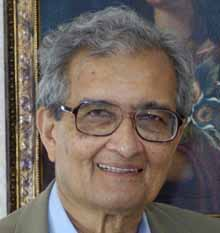
\includegraphics[width=0.5\linewidth]{sen.jpg}
		
		\column{0.6\textwidth}
			\begin{itemize}
				\item[-] Amartya Sen, 1998 Nobel Price in economic science
				\item[-] In his book \textit{Poverty and Famine} he mentioned an entitlement theory. \citep{sen1982poverty}
			\end{itemize}
	  \end{columns}
\end{frame}

\begin{frame}{Why Irish Starving?}
	Amartya only find evidence in India, the Great Bengal Famine, so I am curious if we can use this theory to analysis Irish situation.
	\begin{itemize}
		\item[-] So the assumption will be it is not because Ireland lack of food, but because Irish can not get the food.
	\end{itemize}
	\rule{\linewidth}{0.3mm}
	[Maybe is a pie in the sky]\\
	\vspace*{.5cm}
	Further, I am going to compare different provinces in Ireland and try to find if this province suffer less stringency in the famine is because people have more right.
\end{frame}

\section{Data}
\begin{frame}{Data Introduction}
	Aiming at time range from 1821 to 1900, I combined data from these old documents:
	\begin{itemize}
		\item[-] Ireland census from 1821 to 1891
		\item[-] Ireland population estimate research
		\item[-] Central Statistics Office 19th century agriculture report
		\item[-] The Irish National Archives of price and yield
		\item[-] Irish Industrail Report 
		\item[-] Ireland Statistics Department 1927 Report
		\item[-] UK 19th century import and export list
		\item[-] \ldots
	\end{itemize}
\end{frame}

\begin{frame}{Data Introduction}
	\begin{itemize}
		\item[-] It looks like this:
	\end{itemize}
	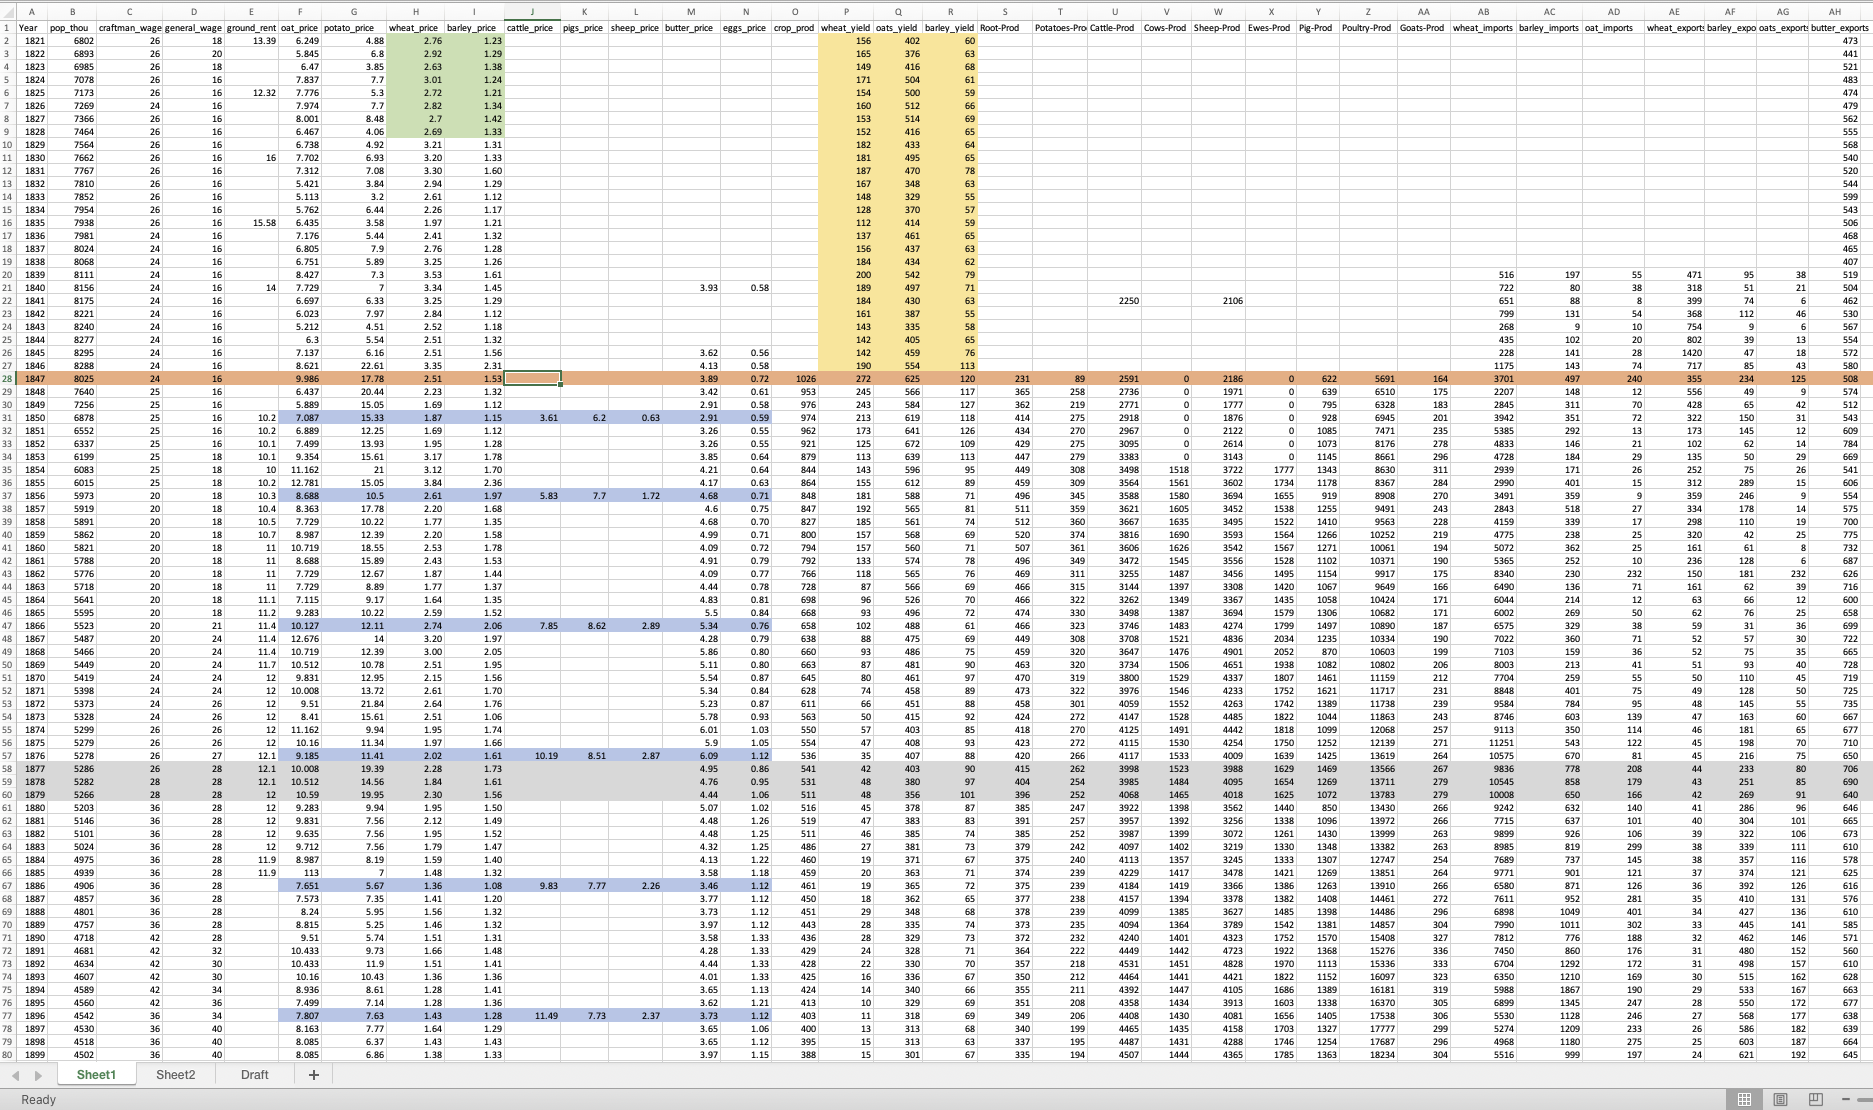
\includegraphics[width=1.05\textwidth]{dataframe_look.png}
\end{frame}

\begin{frame}{Population}
	\begin{itemize}
		\item[-] I used Ireland 1821 to 1891 census and immigration estimation to calculate the 19th century population.
	\end{itemize}
	\begin{center}
		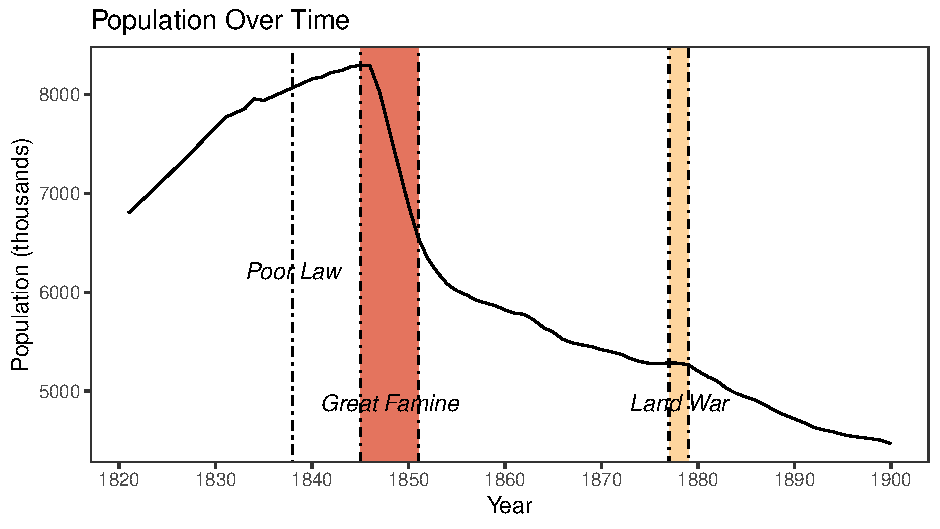
\includegraphics[width=1\textwidth]{population.pdf}
	\end{center}

\end{frame}

\begin{frame}{Wage}
	\begin{itemize}
		\item[-] I used the lowest wage in Dublin to estimate the average wage in Ireland.
	\end{itemize}
	\begin{center}
	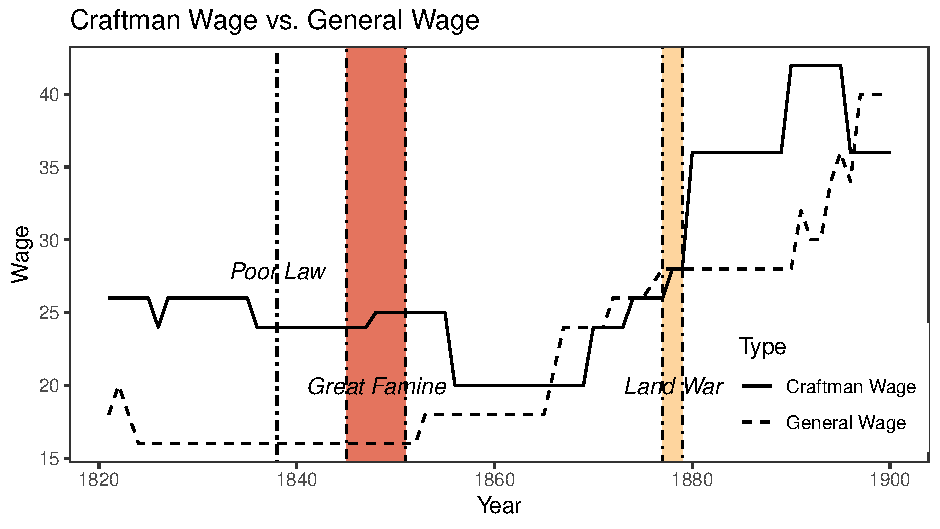
\includegraphics[width=1\textwidth]{wage.pdf}
	\end{center}
\end{frame}

\begin{frame}{Grain Prices}
	\begin{itemize}
		\item[-] Barley, oat, potato and wheat were the four main grain in 19th century's Ireland (Maybe till today).
	\end{itemize}
	\begin{center}
	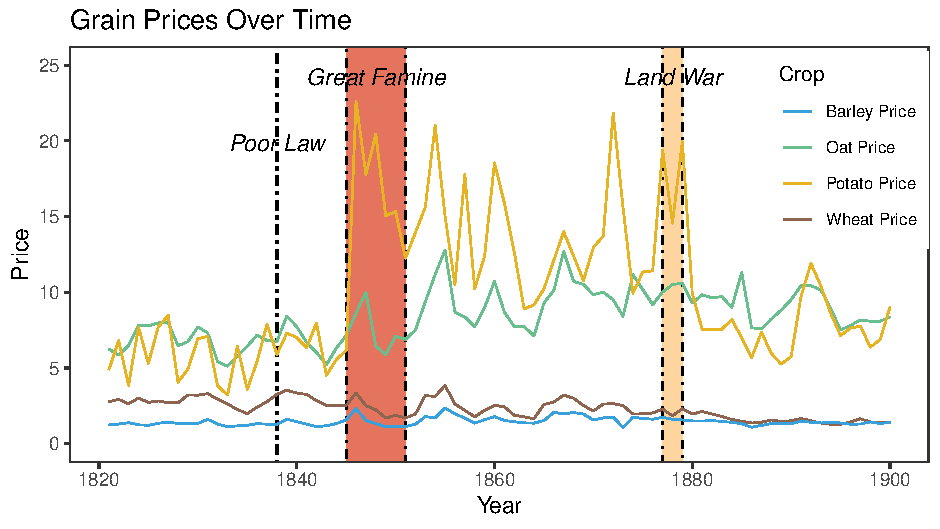
\includegraphics[width=1\textwidth]{grainprice.pdf}
	\end{center}
\end{frame}

\begin{frame}{Potato Price \& Oats Price}
	\begin{itemize}
		\item[-] Potato and Oats were two most yield in nineteenth century.
	\end{itemize}
	\begin{center}
	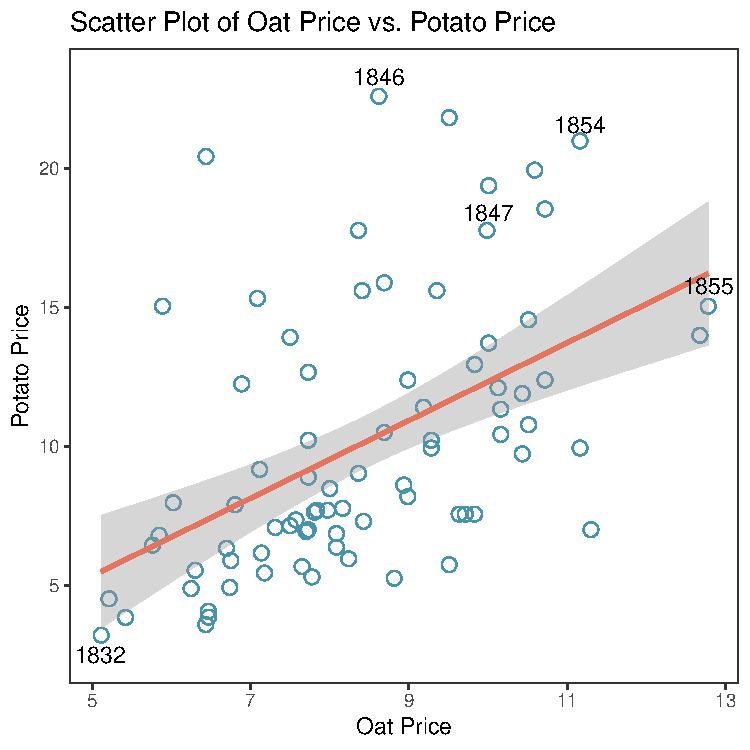
\includegraphics[width=.65\textwidth]{pricecatter.pdf}
	\end{center}
\end{frame}

\begin{frame}{Other Things}
	I am still working on this data set, here are things I already known but not draw a plot in this presentation:
	\begin{itemize}
		\item[-] Grain yield (wheats, oats, barley and livestock numbers from 1847)
		\item[-] Eggs and buttery price from 1845 
		\item[-] Grain import and export from 1839, butter export from 1821
	\end{itemize}
	Here are things I need to know more: 
	\begin{itemize}
		\item[-] Ground rent and taxes from 1821 to 1900
		\item[-] More details about livestock price and yield 
		\item[-] \ldots 
	\end{itemize}
\end{frame}

\section{Research Methods}
\begin{frame}{Regression}
	Maybe there are two regression approaches:
	\begin{itemize}
		\item[-] A RDD regression will be conducted to see if the people's entitlement change around the famine cutoff.
		\item[-] A regression model will be conducted to see which contribute to the population decrease more, food or right?
	\end{itemize}
	\vspace*{.5cm}
	Also, I already found a poverty index and population index in 1847 of the east and west part of Ireland. So I am planning to use this spatial data to analysis the relationship between poverty and famine.
\end{frame}

\begin{frame}
	\bibliographystyle{agsm}
	\bibliography{mybibliography}
\end{frame}

\end{document}


